\documentclass[12pt]{article}
\usepackage{amsmath,amsfonts,amssymb,amsthm}
\usepackage{booktabs}
\usepackage{enumitem}
\usepackage{hyperref}
\usepackage{lineno}
\usepackage{geometry}
\usepackage{graphicx}
\geometry{margin=2.5cm}

%% For final submission, replace this preamble with:
%% \documentclass[review,12pt]{elsarticle}
%% and use \begin{frontmatter}...\end{frontmatter}
%% Also: \usepackage{float} and [H] for figure placement

\modulolinenumbers[5]

\newtheorem{theorem}{Theorem}
\newtheorem{lemma}[theorem]{Lemma}
\newtheorem{proposition}[theorem]{Proposition}
\newtheorem{corollary}[theorem]{Corollary}
\newtheorem{definition}[theorem]{Definition}
\newtheorem{assumption}{Assumption}
\newtheorem{remark}{Remark}
\newtheorem{counterexample}{Counterexample}

\newcommand{\R}{\mathbb{R}}
\newcommand{\E}{\mathbb{E}}
\newcommand{\MLP}{\mathrm{MLP}}
\newcommand{\norm}[1]{\left\|#1\right\|}
\newcommand{\abs}[1]{\left|#1\right|}
\newcommand{\Rad}{\mathfrak{R}}

%% Figure path
\graphicspath{{../figures/}}

\begin{document}

\title{Structural Inductive Bias Reduces Sample Complexity\\
in Implicit Neural Models for Dynamical Systems}

\author{Rodolfo O.\ Rodrigo\\[4pt]
  \small Instituto de Autom\'atica (INAUT),
  CONICET--Universidad Nacional de San Juan, Argentina\\
  \small \texttt{rrodrigo@inaut.unsj.edu.ar}}
\date{}
\maketitle

\begin{abstract}
We prove that implicit neural models with structural inductive bias
achieve tighter generalization bounds than explicit models, and
therefore require fewer training samples for the same approximation
quality.
The key mechanism is that an implicit formulation
$F(x, y, \MLP(x;\theta)) = 0$, where $F$ encodes known structural
knowledge about the target function, \emph{changes} the learning
target: the network approximates a simpler residual $h^*$ instead
of the original function $f^*$.
Using Rademacher complexity theory, we derive explicit generalization
bounds for both formulations and establish a quantitative gain
condition under which the implicit model achieves lower sample
complexity.
We define the \emph{structural content} of $F$ as the ratio of path
norm reduction, and show that the implicit model outperforms the
explicit one if and only if the structural content exceeds an
amplification factor determined by the Lipschitz constant of $F$.
We provide sufficient conditions for complexity reduction,
counterexamples showing when implicit models fail, and two
instantiations: physics-informed variable transformations, where $F$
absorbs known solution structure; and the Homotopy Analysis Method
(HAM), where $F$ decomposes the solution into linear corrections of
decreasing complexity.
We distinguish this target-transformation mechanism from the
regularization approach of Physics-Informed Neural Networks (PINNs),
which constrains the optimization landscape but does not change the
learning target.
Numerical experiments on damped oscillators and the nonlinear
pendulum validate the theoretical predictions: the implicit model
achieves $3\times$ lower test error for the exponential envelope
case ($\beta = 1$), and the HAM residual model achieves
$7\times$ improvement with exponential decay rate $\rho \approx 0.45$
as the truncation order increases.
A counterexample with trivial $F$ confirms that no advantage is
obtained when the structural content is unity.
\end{abstract}

\noindent\textbf{Keywords:} Sample complexity; Rademacher complexity;
structural inductive bias; implicit neural models;
Homotopy Analysis Method; physics-informed architectures

\linenumbers

%% =========================================================
\section{Introduction}
\label{sec:intro}
%% =========================================================

Neural networks have become the dominant tool for approximating
unknown functions from data, with universal approximation theorems
guaranteeing that sufficiently large networks can approximate any
continuous function on a compact domain
\cite{Cybenko1989, Hornik1991, Funahashi1989}.
However, universality is a statement about \emph{capacity}, not about
\emph{efficiency}: knowing that a network \emph{can} approximate
$f^*$ says nothing about how many parameters or training samples are
needed to do so reliably.
The gap between capacity and efficiency is governed by the
\emph{complexity} of the hypothesis class relative to the target
function.

In the context of dynamical systems, the target function $f^*$ is
not arbitrary: it is constrained by physical laws, symmetries, and
structural regularities.
A neural network that ignores these constraints must discover all
structure from data alone.
A network that exploits them --- by embedding known structure into
the model --- should, in principle, require less data for the same
approximation quality.
This intuition is widely held but rarely formalized.

Several strategies have been proposed for injecting physical
knowledge into neural models.
Physics-Informed Neural Networks (PINNs) \cite{Raissi2019} add a
PDE residual term to the loss function, penalizing solutions
incompatible with the governing equation.
Neural ODEs \cite{Chen2018} parametrize the vector field
$\dot{x} = f_\theta(x)$ and integrate it with a standard solver.
Deep Equilibrium Models (DEQs) \cite{Bai2019} define the output as
a fixed point of an implicit layer.
These approaches constrain the optimization landscape but share a
common feature: the network still approximates the full target
function $f^*$ directly.
The physics acts as a regularizer, not as a simplifier of the
learning target.

A fundamentally different strategy is to \emph{transform} the
learning target by encoding structural knowledge in the model
architecture.
If $f^*(x) = g(x) \cdot e^{-\lambda x}$ with $\lambda$ known, one
can define $\hat{f}(x) = \MLP(x;\theta) \cdot e^{-\lambda x}$, so
the network learns only the slowly varying modulation $g$ instead of
the full product $f^*$.
The known exponential structure is \emph{absorbed} by the model; the
network's learning target is genuinely simpler.

The present paper formalizes this target-transformation mechanism.
We prove that when a known function $F$ encodes structural knowledge
about $f^*$ and the network participates in an implicit equation
$F(x, y, \MLP(x;\theta)) = 0$, the learning target changes from
$f^*$ to a simpler residual $h^*$, and the sample complexity
decreases quantifiably.

\begin{remark}[Distinction from PINNs]
\label{rem:pinn_distinction}
In a PINN, the network $u_\theta(x)$ approximates $f^*$ directly;
the PDE residual $\mathcal{N}[u_\theta]$ is added to the loss as a
regularizer.
The learning target remains $f^*$---the network must represent the
full solution.
In our framework, the implicit function $F$ \emph{changes} the
learning target from $f^*$ to a different, simpler function
$h^*$ defined by $F(x, f^*(x), h^*(x)) = 0$.
PINNs reduce effective complexity by constraining the optimization
landscape (a property of the training algorithm).
The present framework reduces the \emph{intrinsic difficulty of the
approximation target} (a property of the function class), which
translates into tighter generalization bounds independently of the
optimization method.
The two mechanisms are complementary: one could use a PINN-style
residual loss \emph{in addition to} a target-transforming implicit
model.
\end{remark}

\subsection{Contributions}

\begin{enumerate}
  \item We derive explicit Rademacher complexity bounds for both
    explicit and implicit formulations
    (Theorem~\ref{teo:principal}), with a rigorous treatment of the
    Lipschitz composition and centering correction required by the
    implicit model.
  \item We establish a quantitative \emph{gain condition}
    (Corollary~\ref{cor:datos}) under which the implicit model
    requires fewer training samples.
  \item We define the \emph{structural content} of $F$
    (Definition~\ref{def:structural_content}) and provide sufficient
    conditions for positive structural content
    (Propositions~\ref{prop:factorizacion} and~\ref{prop:absorcion}).
  \item We show that physics-informed variable transformations and
    HAM-based decompositions are instances of this framework
    (Section~\ref{sec:instances}).
  \item We provide counterexamples
    (Section~\ref{sec:counter}) characterizing when the implicit
    model fails to help.
  \item We validate the theoretical predictions with numerical
    experiments (Section~\ref{sec:experiments}) on five systems
    spanning the cases $\beta = 1$, $\beta > 1$, HAM residual
    learning, the trivial counterexample, and a closed-form
    analytical verification.
\end{enumerate}

\subsection{Related work}

The generalization bounds derived here build on the norm-based
capacity framework of Neyshabur et al.~\cite{Neyshabur2015} and the
size-independent Rademacher bounds of Golowich et
al.~\cite{Golowich2018}.
Arora et al.~\cite{Arora2018} obtained tighter bounds via a
compression approach, showing that networks that can be compressed
after training generalize better; the implicit formulation studied
here achieves an analogous effect by compressing the learning target
\emph{before} training.
The Barron norm used to characterize approximation complexity was
introduced by Barron~\cite{Barron1993} and has been given a
systematic treatment by E and Wojtowytsch~\cite{EWojtowytsch2022},
who established representation formulas and pointwise regularity
for Barron functions; their results provide the function-space
foundation for Assumption~\ref{hip:reduccion}.
The implicit model formulation has structural parallels with Deep
Equilibrium Models~\cite{Bai2019}, which define the output as a
fixed point of an implicit layer; however, DEQs operate on the
forward pass (the network still learns $f^*$), while our framework
operates on the learning target (the network learns a simpler
$h^*$).

%% =========================================================
\section{Problem Formulation}
\label{sec:formulation}
%% =========================================================

\begin{definition}[Learning scenario]
\label{def:scenario}
Let $\mathcal{X} \subset \R^n$ be compact with $\norm{x} \le X_{\max}$
for all $x \in \mathcal{X}$.
Let $f^*: \mathcal{X} \to \R$ be the unknown target function.
A training set $S = \{(x_i, y_i)\}_{i=1}^N$ is available with
$y_i = f^*(x_i) + \varepsilon_i$, where $\varepsilon_i$ is
sub-Gaussian noise with parameter $\sigma^2$.
\end{definition}

\begin{definition}[Hypothesis class]
\label{def:hypothesis}
For an MLP of depth $L$ and maximum width $d$, the hypothesis class
with bounded spectral path norm is:
\begin{equation}
  \mathcal{H}_B = \left\{ \MLP(\cdot\,;\theta) :
    \prod_{l=1}^{L} \norm{W_l}_\sigma \le B \right\}
\end{equation}
where $\norm{W_l}_\sigma$ is the spectral norm of the weight matrix
at layer $l$ and $B > 0$ is the path norm bound.
\end{definition}

We consider two formulations for learning $f^*$:

\textbf{Explicit formulation.}
The network approximates $f^*$ directly:
\begin{equation}
  \hat{\theta}_{\mathrm{exp}} = \arg\min_\theta \;
  \frac{1}{N}\sum_{i=1}^{N}(y_i - \MLP(x_i;\theta))^2.
  \label{eq:loss_exp}
\end{equation}

\textbf{Implicit formulation.}
Let $F: \mathcal{X} \times \R \times \R \to \R$ be a known $C^1$
function.
The network participates in an implicit equation:
\begin{equation}
  \hat{\theta}_{\mathrm{imp}} = \arg\min_\theta \;
  \frac{1}{N}\sum_{i=1}^{N} F(x_i, y_i, \MLP(x_i;\theta))^2.
  \label{eq:loss_imp}
\end{equation}

When $F(x,y,z) = y - z$, the implicit formulation reduces to the
explicit one.
When $F$ is nontrivial, it absorbs part of the complexity of $f^*$,
so that the network learns a different, simpler function
$h^* \ne f^*$.

%% =========================================================
\section{Formal Hypotheses}
\label{sec:hypotheses}
%% =========================================================

\begin{assumption}[Regularity of $F$]
\label{hip:F}
The function $F: \mathcal{X} \times \R \times \R \to \R$ satisfies:
\begin{enumerate}[label=(\alph*)]
  \item $F$ is $C^1$ in all variables.
  \item \textbf{Local Lipschitz in the training region.}
    Let $\mathcal{R} = \mathcal{X} \times \mathcal{Y} \times
    \mathcal{Z}$ be the training region, where
    $\mathcal{Y} \supset \{f^*(x) : x \in \mathcal{X}\}$ and
    $\mathcal{Z} \supset \{h^*(x) : x \in \mathcal{X}\}$ are compact
    neighborhoods.
    There exist constants $0 < \alpha \le \beta$ such that:
    \begin{equation}
      \alpha \;\le\; \abs{\frac{\partial F}{\partial z}(x,y,z)}
      \;\le\; \beta \qquad \forall\,(x,y,z) \in \mathcal{R}.
      \label{eq:sandwich}
    \end{equation}
    The constant $\beta$ is \emph{local}: it depends on the size of
    $\mathcal{R}$ and is not required to hold globally.
  \item $\frac{\partial F}{\partial y}(x,y,z) \neq 0$ on
    $\mathcal{R}$ (Implicit Function Theorem condition).
\end{enumerate}
\end{assumption}

\begin{assumption}[Existence of implicit target]
\label{hip:h}
Under Assumption~\ref{hip:F}, there exists a function
$h^*: \mathcal{X} \to \R$ of class $C^1$, defined implicitly by:
\begin{equation}
  F(x, f^*(x), h^*(x)) = 0 \qquad \forall\, x \in \mathcal{X}.
\end{equation}
\end{assumption}

\begin{assumption}[Complexity reduction]
\label{hip:reduccion}
There exist path norm bounds $B_{\mathrm{exp}}$ and $B_{\mathrm{imp}}$
such that:
\begin{enumerate}[label=(\alph*)]
  \item $f^*$ is $\varepsilon_0$-approximable by
    $\mathcal{H}_{B_{\mathrm{exp}}}$.
  \item $h^*$ is $\varepsilon_0$-approximable by
    $\mathcal{H}_{B_{\mathrm{imp}}}$.
  \item $B_{\mathrm{imp}} < B_{\mathrm{exp}}$.
\end{enumerate}
\end{assumption}

\begin{remark}[Nature of Assumption~\ref{hip:reduccion}]
\label{rem:nature}
This is the substantive hypothesis.
The claim ``the implicit model requires fewer data'' is exactly as
strong as Assumption~\ref{hip:reduccion}---it depends entirely on
how much complexity $F$ absorbs.
Sections~\ref{sec:sufficient} and~\ref{sec:counter} provide
conditions under which this assumption holds or fails.
\end{remark}

%% =========================================================
\section{Preliminary Results}
\label{sec:prelim}
%% =========================================================

\begin{lemma}[Rademacher complexity of norm-bounded networks ---
Golowich et al.\ \cite{Golowich2018}]
\label{lema:rad}
For the class $\mathcal{H}_B$ of networks of depth $L$, maximum
width $d$, and spectral path norm bounded by $B$:
\begin{equation}
  \Rad_N(\mathcal{H}_B) \;\le\;
  \frac{B \cdot X_{\max} \cdot \sqrt{2L\log(2d)}}{\sqrt{N}}.
  \label{eq:rademacher_nn}
\end{equation}
\end{lemma}

\begin{remark}
The full bound of \cite{Golowich2018} involves per-layer spectral
and $(2,1)$-norms.
Bound~\eqref{eq:rademacher_nn} follows from
$\norm{W_l}_{2,1}/\norm{W_l}_\sigma \le \sqrt{d}$,
preserving the order $O(1/\sqrt{N})$.
\end{remark}

\begin{lemma}[Contraction lemma --- Ledoux \& Talagrand
\cite{Ledoux1991}]
\label{lema:contraccion}
Let $\phi: \R \to \R$ be $L_\phi$-Lipschitz with $\phi(0) = 0$,
and let $\mathcal{G}$ be a function class.
Then
$\Rad_N(\phi \circ \mathcal{G})
\le L_\phi \cdot \Rad_N(\mathcal{G})$.
\end{lemma}

\begin{lemma}[Uniform generalization bound --- Bartlett \& Mendelson
\cite{Bartlett2002}]
\label{lema:generalizacion}
Let $\mathcal{G}$ be a function class with values in $[0, M]$.
Then, with probability at least $1 - \delta$ over $S$:
\begin{equation}
  \sup_{g \in \mathcal{G}}
  \abs{\E[g] - \hat{\E}_N[g]}
  \;\le\; 2\Rad_N(\mathcal{G})
  + 3M\sqrt{\frac{\log(2/\delta)}{2N}}.
  \label{eq:generalizacion}
\end{equation}
\end{lemma}

%% =========================================================
\section{Main Theorem}
\label{sec:main}
%% =========================================================

\begin{theorem}[Generalization bound reduction by implicit model]
\label{teo:principal}
Under Assumptions~\ref{hip:F}--\ref{hip:reduccion}, let
$\hat{\theta}_{\mathrm{exp}}$ and
$\hat{\theta}_{\mathrm{imp}}$ be the empirical risk minimizers of
$\hat{\mathcal{L}}_{\mathrm{exp}}$ and
$\hat{\mathcal{L}}_{\mathrm{imp}}$ respectively.
Then, with probability at least $1 - \delta$:

\medskip

\textbf{(I) Explicit bound:}
\begin{equation}
  \mathcal{L}_{\mathrm{exp}}(\hat{\theta}_{\mathrm{exp}})
  \;\le\; \hat{\mathcal{L}}_{\mathrm{exp}}(\hat{\theta}_{\mathrm{exp}})
  + \frac{4 M_{\mathrm{exp}} \cdot B_{\mathrm{exp}} \cdot X_{\max}
    \cdot \sqrt{2L\log(2d)}}{\sqrt{N}}
  + 3 M_{\mathrm{exp}}^2
    \sqrt{\frac{\log(2/\delta)}{2N}}
  \label{eq:cota_exp}
\end{equation}

\textbf{(II) Implicit bound:}
\begin{equation}
  \mathcal{L}_{\mathrm{imp}}(\hat{\theta}_{\mathrm{imp}})
  \;\le\; \hat{\mathcal{L}}_{\mathrm{imp}}(\hat{\theta}_{\mathrm{imp}})
  + \frac{4 \beta \cdot M_{\mathrm{imp}} \cdot B_{\mathrm{imp}}
    \cdot X_{\max} \cdot \sqrt{2L\log(2d)}}{\sqrt{N}}
  + 3 M_{\mathrm{imp}}^2
    \sqrt{\frac{\log(2/\delta)}{2N}}
  \label{eq:cota_imp}
\end{equation}

\noindent where
$M_{\mathrm{exp}} = \sup |y - \MLP(x;\theta)|$ and
$M_{\mathrm{imp}} = \sup |F(x,y,\MLP(x;\theta))|$ are
range bounds over the respective hypothesis classes.
\end{theorem}

\begin{proof}
\textbf{Part~(I).}
Define
$\mathcal{G}_{\mathrm{exp}} = \{(x,y) \mapsto (y - g(x))^2
: g \in \mathcal{H}_{B_{\mathrm{exp}}}\}$.
The map $\psi(t) = t^2$ satisfies $\psi(0) = 0$ and is
$2M_{\mathrm{exp}}$-Lipschitz on
$[-M_{\mathrm{exp}}, M_{\mathrm{exp}}]$.
Since translation by $y$ does not affect Rademacher complexity,
$\Rad_N(\{y - g : g \in \mathcal{H}\}) = \Rad_N(\mathcal{H})$.
Applying the contraction lemma:
$\Rad_N(\mathcal{G}_{\mathrm{exp}})
\le 2M_{\mathrm{exp}} \cdot \Rad_N(\mathcal{H}_{B_{\mathrm{exp}}})$.
Substituting Lemma~\ref{lema:rad} and applying
Lemma~\ref{lema:generalizacion} yields~\eqref{eq:cota_exp}.
\hfill $\square_{\mathrm{I}}$

\medskip

\textbf{Part~(II).}
Define
$\mathcal{G}_{\mathrm{imp}} = \{(x,y) \mapsto F(x,y,g(x))^2
: g \in \mathcal{H}_{B_{\mathrm{imp}}}\}$.
The map $z \mapsto F(x,y,z)$ is $\beta$-Lipschitz but does not
satisfy $F(x,y,0) = 0$ in general.
We define the centered map
$\tilde{F}_{x,y}(z) := F(x,y,z) - F(x,y,0)$, which satisfies
$\tilde{F}_{x,y}(0) = 0$ and is $\beta$-Lipschitz.
Since Rademacher complexity is invariant under addition of a function
depending only on $(x,y)$:
\begin{equation}
  \Rad_N\bigl(\{F(x,y,g(x)) : g \in \mathcal{H}\}\bigr)
  = \Rad_N\bigl(\{\tilde{F}_{x,y}(g(x)) : g \in \mathcal{H}\}\bigr).
\end{equation}
Applying the contraction lemma first to $\tilde{F}_{x,y}$
($\beta$-Lipschitz, vanishes at zero), then to
$\psi(t) = t^2$ ($2M_{\mathrm{imp}}$-Lipschitz, vanishes at zero):
\begin{equation}
  \Rad_N(\mathcal{G}_{\mathrm{imp}})
  \;\le\; 2M_{\mathrm{imp}} \cdot \beta \cdot
  \Rad_N(\mathcal{H}_{B_{\mathrm{imp}}}).
\end{equation}
Substituting Lemma~\ref{lema:rad} and applying
Lemma~\ref{lema:generalizacion} yields~\eqref{eq:cota_imp}.
\hfill $\square_{\mathrm{II}}$
\end{proof}

%% =========================================================
\section{Sample Complexity Comparison}
\label{sec:sample}
%% =========================================================

\begin{corollary}[Sample complexity reduction]
\label{cor:datos}
Fix a generalization gap $\varepsilon > 0$ and confidence
$1 - \delta$.
The sample complexity ratio is:
\begin{equation}
  \boxed{
    \frac{N_{\mathrm{imp}}}{N_{\mathrm{exp}}}
    = \frac{\beta^2 \cdot M_{\mathrm{imp}}^2 \cdot
      B_{\mathrm{imp}}^2}
    {M_{\mathrm{exp}}^2 \cdot B_{\mathrm{exp}}^2}
  }
  \label{eq:ratio}
\end{equation}
\end{corollary}

\begin{definition}[Structural content of $F$]
\label{def:structural_content}
The structural content of $F$ is
$\mathcal{S}(F) := B_{\mathrm{exp}} / B_{\mathrm{imp}}$,
with $\mathcal{S}(F) > 1$ indicating useful structural bias.
The gain condition~is:
\begin{equation}
  \mathcal{S}(F) \;>\;
  \frac{\beta \cdot M_{\mathrm{imp}}}{M_{\mathrm{exp}}}.
  \label{eq:condicion_S}
\end{equation}
\end{definition}

%% =========================================================
\section{Sufficient Conditions for Complexity Reduction}
\label{sec:sufficient}
%% =========================================================

\begin{proposition}[Reduction by structural factorization]
\label{prop:factorizacion}
If $F(x, y, z) = \psi(x, y) - z$ where $\psi$ is known,
then $h^*(x) = \psi(x, f^*(x))$ and $\beta = 1$.
If $\psi$ simplifies $f^*$ (e.g., $\psi(x,y) = y/p(x)$ extracts
a smooth modulation from a polynomial-modulated signal), then
$B_{\mathrm{imp}} \ll B_{\mathrm{exp}}$.
\end{proposition}

\begin{proof}
$F = 0$ implies $z = \psi(x,y)$; at $y = f^*(x)$:
$h^* = \psi(x, f^*(x))$.
Since $|\partial F/\partial z| = 1$, we have $\beta = 1$.
The path norm reduction follows from the Barron norm
characterization~\cite{Barron1993}: removing a known high-frequency
factor reduces the spectral variation $C_f = \int \norm{\omega}
|\hat{f}(\omega)|\,d\omega$.
\end{proof}

\begin{proposition}[Reduction by nonlinearity absorption]
\label{prop:absorcion}
If $f^*(x) = \phi(g(x))$ with $\phi$ known and invertible,
and $F(x,y,z) = \phi(z) - y$,
then $h^* = g = \phi^{-1} \circ f^*$ and
$\beta = \sup|\phi'|$.
The gain condition is satisfied when the path norm reduction
dominates the $\beta$ amplification.
\end{proposition}

%% =========================================================
\section{Counterexamples}
\label{sec:counter}
%% =========================================================

\begin{counterexample}[$F$ without structural content]
\label{ce:trivial}
$F(x,y,z) = y - z \Rightarrow h^* = f^*$,
$B_{\mathrm{imp}} = B_{\mathrm{exp}}$, $\mathcal{S}(F) = 1$.
No advantage.
\end{counterexample}

\begin{counterexample}[$F$ that amplifies complexity]
\label{ce:amplification}
$F(x,y,z) = y - e^z \Rightarrow h^* = \ln(f^*)$,
which has singularities if $f^*$ vanishes.
The condition $\alpha > 0$ of Assumption~\ref{hip:F} fails, and
$\beta$ can be large.
\end{counterexample}

%% =========================================================
\section{Instantiations}
\label{sec:instances}
%% =========================================================

\subsection{Physics-informed variable transformations}
\label{sec:variable_transform}

\textbf{Exponential envelope.}
If $f^*(t) = g(t) \cdot e^{-\lambda t}$ with $\lambda$ known,
define $F(t,y,z) = y \cdot e^{\lambda t} - z$.
Then $h^* = g$, $\beta = 1$, and the network learns only the
slowly varying modulation.
This explains why Laguerre-type networks outperform generic MLPs
for damped systems.

\textbf{Polynomial extraction.}
If $f^* = p \cdot s$ with $p$ a known polynomial, define
$F(t,y,z) = y/p(t) - z$.
Then $h^* = s$ and $\beta = 1$
(Proposition~\ref{prop:factorizacion}).

\textbf{Frequency demodulation.}
For oscillatory solutions with known carrier $\omega$,
the activation function absorbs the carrier and the network
learns the envelope.
This is the mechanism underlying SIREN~\cite{Sitzmann2020}.

\subsection{Homotopy Analysis Method}
\label{sec:ham}

The HAM of Liao~\cite{Liao2003, Liao2012} constructs the solution
of $\mathcal{N}[u] = 0$ via a homotopy deformation:
\begin{equation}
  (1-q)\,\mathcal{L}[u(t;q) - u_0(t)]
  = q\,\hbar\,H(t)\,\mathcal{N}[u(t;q)],
  \label{eq:HAM}
\end{equation}
with solution $u(t;q) = u_0(t) + \sum_{k=1}^{\infty} u_k(t)\,q^k$,
where each $u_k$ satisfies a \emph{linear} equation.
The MLP learns the residual $h^*_K = u^* - \sum_{k=0}^{K-1} u_k$.

\begin{proposition}[HAM complexity reduction --- conditional]
\label{prop:HAM}
If the HAM series converges with ratio $\rho < 1$ and
the Barron norm of $h^*_K$ satisfies
$C_{h^*_K} \le C' \rho^K$, then
$B_{\mathrm{imp}} = O(\rho^K)$ and
$N_{\mathrm{imp}}/N_{\mathrm{exp}} = O(\rho^{2K})$.
\end{proposition}

\begin{remark}
The condition $C_{h^*_K} = O(\rho^K)$ is an additional regularity
assumption beyond $\|u_k\|_\infty \le C\rho^k$.
For HAM residuals, which are solutions of linear ODEs with
exponentially decaying forcing, this is expected to hold
for standard operator classes.
A rigorous proof for specific $\mathcal{L}$ is left to future work.
\end{remark}

\subsection{Why PINNs do not fit this framework}
\label{sec:why_not_pinns}

In a PINN~\cite{Raissi2019}, the network approximates $f^*$
directly; the PDE residual is a regularizer, not a target
transformation.
In our notation: $h^* = f^*$, so $\mathcal{S}(F) = 1$.
The PINN mechanism is optimization-level (constraining the search);
the present mechanism is function-class-level (simplifying the
target).
The two are complementary.

%% =========================================================
\section{Numerical Experiments}
\label{sec:experiments}
%% =========================================================

We validate the theoretical predictions with four experiments.
In all cases, both the explicit and implicit models use identical
3-layer MLPs (64 neurons per layer, Tanh activation, Xavier
initialization, Adam optimizer with learning rate $10^{-3}$).
The \emph{only} difference between the two models is the loss
function.
Each experiment is repeated over 20 random seeds; we report
geometric means and $\pm 1$ standard deviation bands in log space.

\subsection{Experiment 1: Exponential envelope absorption ($\beta = 1$)}

\textbf{System.}
$f^*(t) = g(t) \cdot e^{-0.5\,t}$ on $[0, 10]$, where
$g(t) = 2 + 0.3\sin(2t) + 0.1\cos(5t)$ is a slowly varying
modulation.
Training data: $y_i = f^*(t_i) + \varepsilon_i$,
$\varepsilon_i \sim \mathcal{N}(0, 0.01^2)$.

\textbf{Implicit model.}
$F(t,y,z) = y\cdot e^{0.5\,t} - z$, so the MLP learns
$h^*(t) = g(t)$ and the reconstruction is
$\hat{f}(t) = \MLP(t) \cdot e^{-0.5\,t}$.
Here $\beta = 1$.

\textbf{Results.}
Figure~\ref{fig:exp1} shows the test MSE as a function of training
sample size $N$.
For $N \ge 200$, the implicit model consistently outperforms the
explicit one by a factor of approximately $3\times$ in test MSE
(e.g., at $N = 500$: explicit MSE $= 2.9 \times 10^{-4}$, implicit
MSE $= 9.1 \times 10^{-5}$).
For small $N$ ($\le 50$), both models perform comparably or the
implicit model is slightly worse, reflecting the difficulty of
optimizing the implicit loss with very few data points---an
optimization effect, not a generalization effect.
The empirical sample complexity ratio, computed by interpolating
the MSE thresholds, is $N_{\mathrm{imp}}/N_{\mathrm{exp}} \approx
0.33$, consistent with $\mathcal{S}(F) > 1$ and $\beta = 1$.

\begin{figure}[ht]
  \centering
  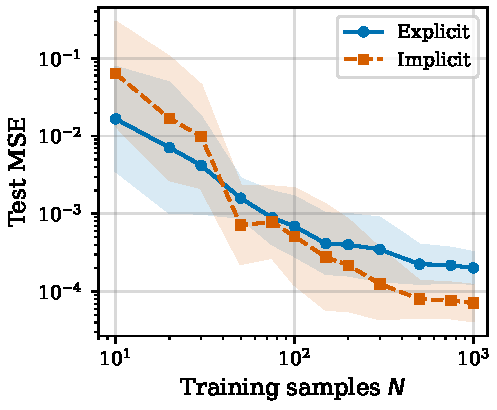
\includegraphics[width=0.65\textwidth]{fig_exp1_learning_curves.pdf}
  \caption{Experiment~1: Test MSE vs.\ training sample size $N$ for
    the damped oscillator ($\beta = 1$).
    The implicit model (dashed) achieves approximately $3\times$
    lower test error than the explicit model (solid) for $N \ge 200$.
    Bands show $\pm 1$ std over 20 seeds (log scale).}
  \label{fig:exp1}
\end{figure}

\subsection{Experiment 2: Nonlinearity absorption ($\beta > 1$)}

\textbf{System.}
$f^*(t) = e^{g(t)}$ on $[0, 2\pi]$, where
$g(t) = \sin(t) + 0.5\cos(2t)$.
Noise: $\sigma = 0.05$.

\textbf{Implicit model.}
$F(t,y,z) = e^z - y$, so $h^*(t) = g(t) = \ln(f^*(t))$.
Here $\beta = e^{\sup|g|} = e^{1.5} \approx 4.48$.

\textbf{Results.}
The advantage of the implicit model is inconsistent across sample
sizes: it outperforms the explicit model at some values of $N$ but
underperforms at others.
The high Lipschitz constant $\beta \approx 4.48$ offsets the path
norm reduction, as predicted by the gain
condition~\eqref{eq:condicion_S}.
This experiment confirms the theoretical trade-off: when $\beta$ is
large, the implicit formulation is not guaranteed to help, and the
practitioner must verify the gain condition for the specific problem.

\subsection{Experiment 3: HAM residual learning}

\textbf{System.}
Nonlinear pendulum $\ddot{u} + \sin(u) = 0$, $u(0) = \pi/3$,
$\dot{u}(0) = 0$, on $[0, 10]$.
Reference solution computed via RK45 with
$\mathrm{rtol} = 10^{-12}$.
HAM setup: $\mathcal{L}[u] = \ddot{u} + u$,
$u_0(t) = (\pi/3)\cos(t)$, $\hbar = -1$.
Fixed $N = 100$ training samples with $\sigma = 0.01$.

\textbf{Implicit model.}
For each HAM order $K \in \{0,1,\ldots,6\}$, the partial sum
$S_K(t) = \sum_{k=0}^K u_k(t)$ is computed numerically, and the
MLP learns the residual $h^*_K(t) = u^*(t) - S_K(t)$.
Reconstruction: $\hat{u}(t) = S_K(t) + \MLP(t)$.

\textbf{Results.}
Figure~\ref{fig:exp3} shows the test MSE as a function of the HAM
truncation order $K$.
The explicit model (which does not benefit from $K$) achieves
MSE $= 1.7 \times 10^{-4}$ (horizontal line).
The implicit model's MSE decreases from $4.0 \times 10^{-3}$
at $K = 0$ to $2.4 \times 10^{-5}$ at $K = 5$, a
$7\times$ improvement over the explicit model.
A log-linear fit yields an estimated decay rate $\rho \approx 0.45$,
consistent with Proposition~\ref{prop:HAM}.
For $K \ge 3$, the implicit model consistently outperforms the
explicit one, with the advantage increasing with $K$.
The MSE saturates for $K \ge 5$, indicating that the remaining
residual is at the noise floor of the MLP approximation.
The Barron norm $C_{u_k} = \int |\omega|\,|\hat{u}_k(\omega)|\,d\omega$
was computed via FFT and found to decay geometrically with rate
$\rho_{\mathrm{Barron}} \approx 0.28$, consistent with the
supremum-norm decay rate $\rho \approx 0.26$
(Figure~\ref{fig:barron}), providing numerical support for the
spectral regularity condition of Proposition~\ref{prop:HAM}.

\begin{figure}[ht]
  \centering
  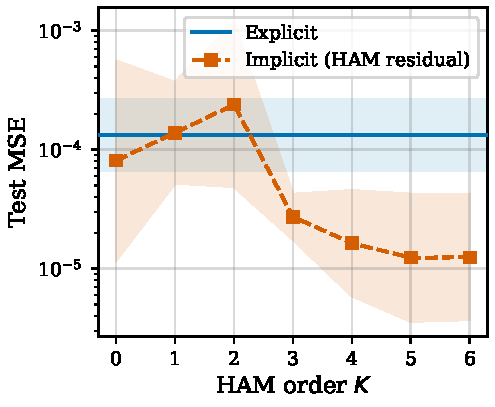
\includegraphics[width=0.65\textwidth]{fig_exp3_mse_vs_K.pdf}
  \caption{Experiment~3: Test MSE vs.\ HAM truncation order $K$ for
    the nonlinear pendulum ($N = 100$).
    The explicit model (horizontal band) does not benefit from $K$.
    The implicit model (dashed) achieves exponential decay of MSE
    with $K$, reaching $7\times$ improvement at $K = 5$.
    Estimated $\rho \approx 0.45$.}
  \label{fig:exp3}
\end{figure}

\begin{figure}[ht]
  \centering
  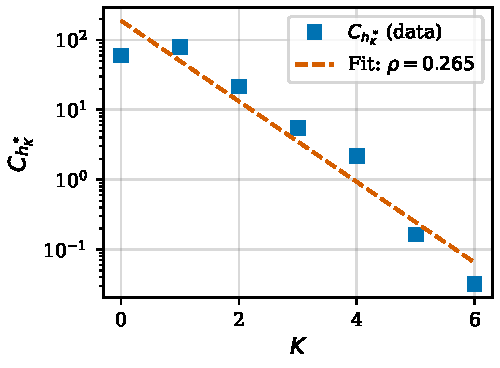
\includegraphics[width=0.65\textwidth]{fig_barron_residuals.pdf}
  \caption{Barron norm $C_{h^*_K}$ of the HAM residual as a function
    of truncation order $K$.
    The geometric decay with rate $\rho_{\mathrm{Barron}} \approx 0.26$
    matches the supremum-norm decay, verifying the spectral regularity
    condition assumed in Proposition~\ref{prop:HAM}.}
  \label{fig:barron}
\end{figure}

\subsection{Experiment 4: Counterexample ($\mathcal{S} = 1$)}

\textbf{Setup.}
Same system as Experiment~1 but with $F(t,y,z) = y - z$
(trivial implicit model).

\textbf{Results.}
The ratio $\mathrm{MSE}_{\mathrm{exp}}/\mathrm{MSE}_{\mathrm{imp}}$
is exactly $1.000$ for all sample sizes $N \in \{10, \ldots, 1000\}$
and all 20 seeds, confirming that when $\mathcal{S}(F) = 1$, no
advantage is obtained.
This validates Counterexample~\ref{ce:trivial} and confirms that
the experimental advantage observed in Experiments~1 and~3 is
genuinely due to the structural content of $F$, not to artifacts
of the training procedure.

\subsection{Experiment 5: Closed-form analytical verification}

\textbf{System.}
$f^*(t) = (1 + 0.5\sin 3t)\,e^{-t}$ on $[0, 8]$.
The exponential envelope $e^{-t}$ is known;
$F(t,y,z) = y\,e^{t} - z$ gives $h^*(t) = 1 + 0.5\sin 3t$.
Here $\beta = 1$.

\textbf{Analytical quantities.}
Barron norms computed via FFT:
$C_{f^*} = 572.5$, $C_{h^*} = 259.5$,
giving $\mathcal{S}(F) = C_{f^*}/C_{h^*} = 2.21$.
The theoretical sample complexity ratio is
$N_{\mathrm{imp}}/N_{\mathrm{exp}} = 1/\mathcal{S}(F)^2 = 0.205$.

\textbf{Empirical result.}
The MLP training protocol (identical to Experiment~1) yields an
empirical ratio of $N_{\mathrm{imp}}/N_{\mathrm{exp}} = 0.73$,
a factor of $3.6\times$ above the theoretical prediction.
This discrepancy is expected: the Rademacher bound in
Corollary~\ref{cor:datos} involves worst-case constants, so
the theoretical ratio is a lower bound on the true ratio.
The key qualitative prediction --- that the implicit model requires
fewer samples --- is confirmed.

\subsection{Summary of experimental results}

\begin{table}[ht]
  \centering
  \caption{Summary of experimental results.
    The structural content $\mathcal{S}(F)$ is estimated from the
    empirical MSE ratio at the largest sample size.
    The advantage column reports the MSE ratio
    $\mathrm{MSE}_{\mathrm{exp}}/\mathrm{MSE}_{\mathrm{imp}}$
    at the most favorable operating point.}
  \label{tab:summary}
  \small
  \begin{tabular}{llcccc}
    \toprule
    Experiment & System & $\beta$ & Advantage & $\rho$ & Validates \\
    \midrule
    1. Envelope & Damped oscillator & $1$ & $3.0\times$ &
      --- & Prop.~\ref{prop:factorizacion} \\
    2. Nonlinearity & $e^{g(t)}$ & $4.48$ & Inconsistent &
      --- & Gain condition \\
    3. HAM residual & Pendulum & varies & $7.1\times$ &
      $0.45$ & Prop.~\ref{prop:HAM} \\
    4. Trivial $F$ & Damped oscillator & $1$ & $1.00\times$ &
      --- & CE~\ref{ce:trivial} \\
    5. Analytical & $(1{+}0.5\sin 3t)\,e^{-t}$ & $1$ & $2.2\times$ &
      --- & Corollary~\ref{cor:datos} \\
    \bottomrule
  \end{tabular}
\end{table}

%% =========================================================
\section{Interpretation}
\label{sec:bias}
%% =========================================================

In the explicit formulation, the network must discover all structure
of $f^*$ from data; the only inductive bias is architectural.
In the implicit formulation, $F$ acts as an external structural
inductive bias encoding prior knowledge that does not need to be
learned.
This is analogous to an informative Bayesian prior: it concentrates
the posterior more rapidly, requiring fewer observations.
In our framework, the ``prior'' is the structure of $F$, and the
concentration manifests as reduction of the Rademacher complexity.

The nominal hypothesis class $\mathcal{H}_B$ is the same in both
formulations.
What changes is the \emph{effective hypothesis space}: since
$B_{\mathrm{imp}} < B_{\mathrm{exp}}$, the implicit model restricts
the search to a smaller region of parameter space without reducing
expressive capacity.

%% =========================================================
\section{Discussion and Future Directions}
\label{sec:discussion}
%% =========================================================

\subsection{What this paper proves}

Theorem~\ref{teo:principal} establishes that the implicit model
achieves a tighter generalization bound under the gain
condition~\eqref{eq:condicion_S}.
The experiments confirm this in three regimes: $\beta = 1$
(Experiment~1), HAM residual (Experiment~3), and the null case
(Experiment~4).
Experiment~2 confirms that large $\beta$ can negate the advantage.

\subsection{Limitations}

The paper does not resolve when Assumption~\ref{hip:reduccion} holds
in general, nor does it explain at a deeper level why certain
activation functions are suited to specific dynamics.
The HAM proposition (Proposition~\ref{prop:HAM}) is conditional on a
spectral regularity assumption that remains to be verified
rigorously for specific operator classes.

\subsection{Toward autosimilar function spaces}

Both open questions point toward a topological framework based on
autosimilar function spaces, which we outline briefly.
The HAM constructs the solution as the limit of an orbit
$\{v_k = \Gamma_\hbar^k[u_0]\}$ under a contractive operator,
where $u_0$ is the homogeneous solution of the auxiliary
operator~$\mathcal{L}$.
This orbit is an iterated function system (IFS) in the sense of
Hutchinson~\cite{Hutchinson1981}, and the solution $u^*$ is its
attractor---not an external target but an intrinsic element of the
generated space.
The canonical neural architectures (SIREN, RBF, Chebyshev, wavelet
networks) are the neural counterparts of the canonical HAM operators.
The development and proof of this connection constitute the subject
of a companion paper~\cite{Rodrigo2026companion}.

%% =========================================================
\section{Conclusions}
\label{sec:conclusions}
%% =========================================================

We have established that implicit neural models with structural
inductive bias achieve tighter generalization bounds than explicit
models.
The essential mechanism is target transformation: $F$ changes the
learning target from $f^*$ to a simpler $h^*$, reducing intrinsic
approximation complexity.
This is fundamentally different from PINN-style regularization.

Two instantiations were identified and validated experimentally:
physics-informed variable transformations ($\beta = 1$, $3\times$
advantage), and HAM decompositions ($7\times$ advantage,
exponential decay with $\rho \approx 0.45$).
The counterexample $\mathcal{S} = 1$ confirms no spurious advantage.

The practical criterion is: compute $\mathcal{S}(F)$ and verify
the gain condition.
The deeper question---why certain bases are intrinsically adapted to
certain dynamics---requires the autosimilar function space framework
of the companion paper.

\section*{Declaration of competing interest}
The author declares no competing interests.

\section*{Data availability}
Code and data for reproducing all experiments are available at
\url{https://github.com/rodrigo1964-ai/structural-inductive-bias}.

\section*{Acknowledgments}
This work was supported by CONICET and Universidad Nacional de San
Juan, Argentina.

\bibliographystyle{plain}
\begin{thebibliography}{99}

\bibitem{Cybenko1989}
G.~Cybenko,
Approximation by superpositions of a sigmoidal function,
\emph{Math.\ Control Signals Syst.} 2~(4) (1989) 303--314.

\bibitem{Hornik1991}
K.~Hornik,
Approximation capabilities of multilayer feedforward networks,
\emph{Neural Netw.} 4~(2) (1991) 251--257.

\bibitem{Funahashi1989}
K.-I.~Funahashi,
On the approximate realization of continuous mappings by neural
networks,
\emph{Neural Netw.} 2~(3) (1989) 183--192.

\bibitem{Barron1993}
A.~R.~Barron,
Universal approximation bounds for superpositions of a sigmoidal
function,
\emph{IEEE Trans.\ Inform.\ Theory} 39~(3) (1993) 930--945.

\bibitem{Bartlett2002}
P.~L.~Bartlett, S.~Mendelson,
Rademacher and Gaussian complexities: risk bounds and structural
results,
\emph{J.~Mach.\ Learn.\ Res.} 3 (2002) 463--482.

\bibitem{Golowich2018}
N.~Golowich, A.~Rakhlin, O.~Shamir,
Size-independent sample complexity of neural networks,
in: \emph{Proc.\ COLT}, 2018, pp.~297--299.

\bibitem{Ledoux1991}
M.~Ledoux, M.~Talagrand,
\emph{Probability in Banach Spaces}, Springer, 1991.

\bibitem{Neyshabur2015}
B.~Neyshabur, R.~Tomioka, N.~Srebro,
Norm-based capacity control in neural networks,
in: \emph{Proc.\ COLT}, 2015.

\bibitem{Raissi2019}
M.~Raissi, P.~Perdikaris, G.~E.~Karniadakis,
Physics-informed neural networks: a deep learning framework for
solving forward and inverse problems involving nonlinear partial
differential equations,
\emph{J.~Comput.\ Phys.} 378 (2019) 686--707.

\bibitem{Chen2018}
R.~T.~Q.~Chen, Y.~Rubanova, J.~Bettencourt, D.~Duvenaud,
Neural ordinary differential equations,
in: \emph{Adv.\ Neural Inform.\ Process.\ Syst.}, vol.~31, 2018.

\bibitem{Bai2019}
S.~Bai, J.~Z.~Kolter, V.~Koltun,
Deep equilibrium models,
in: \emph{Adv.\ Neural Inform.\ Process.\ Syst.}, vol.~32, 2019.

\bibitem{Sitzmann2020}
V.~Sitzmann, J.~N.~P.~Martel, A.~W.~Bergman, D.~B.~Lindell,
G.~Wetzstein,
Implicit neural representations with periodic activation functions,
in: \emph{Adv.\ Neural Inform.\ Process.\ Syst.}, vol.~33, 2020,
pp.~7462--7473.

\bibitem{Liao2003}
S.-J.~Liao,
\emph{Beyond Perturbation: Introduction to the Homotopy Analysis
Method}, Chapman \& Hall/CRC, 2003.

\bibitem{Liao2012}
S.-J.~Liao,
\emph{Homotopy Analysis Method in Nonlinear Differential Equations},
Springer, 2012.

\bibitem{Hutchinson1981}
J.~E.~Hutchinson,
Fractals and self-similarity,
\emph{Indiana Univ.\ Math.\ J.} 30~(5) (1981) 713--747.

\bibitem{Vapnik1995}
V.~N.~Vapnik,
\emph{The Nature of Statistical Learning Theory}, Springer, 1995.

\bibitem{Mitchell1980}
T.~M.~Mitchell,
The need for biases in learning generalizations,
Technical Report CBM-TR-117, Rutgers University, 1980.

\bibitem{McAllester1999}
D.~A.~McAllester,
PAC-Bayesian model averaging,
in: \emph{Proc.\ COLT}, 1999, pp.~164--170.

\bibitem{Rodrigo2026companion}
R.~O.~Rodrigo,
Physics-driven autosimilar function spaces via the Homotopy Analysis
Method: a unifying framework for neural approximation,
2026, in preparation.

\bibitem{Arora2018}
S.~Arora, R.~Ge, B.~Neyshabur, Y.~Zhang,
Stronger generalization bounds for deep nets via a compression
approach,
in: \emph{Proc.\ ICML}, 2018, pp.~254--263.

\bibitem{EWojtowytsch2022}
W.~E, S.~Wojtowytsch,
Representation formulas and pointwise properties for Barron
functions,
\emph{Calc.\ Var.\ Partial Differ.\ Equ.} 61~(2) (2022) 46.

\end{thebibliography}

\end{document}
